\documentclass[10pt,conference]{IEEEtran}

\usepackage{booktabs}
\usepackage{graphicx}
\usepackage{hyperref}
\usepackage{amsmath}
\usepackage{xcolor}
\usepackage{url}

\title{DiffAudit: Evidence-Contracted Membership Leakage Auditing for Diffusion Models}

\author{\IEEEauthorblockN{Anonymous Authors}}

\begin{document}
\maketitle

\begin{abstract}
Membership inference against diffusion models is often reported as a scalar
score, yet a deployable privacy audit needs more than a high AUC. The score
must be tied to a fixed target model, a member/nonmember split, row-level score
or response coverage, reproducible metrics, provenance, and a clear consumer
boundary. We present DiffAudit, an evidence-contracted audit methodology for
diffusion-model membership leakage. DiffAudit separates admitted evidence from
research candidates and watch items, reports finite-tail low-FPR metrics with
their packet denominators, and rejects attractive results whose artifacts do not
support the claimed audit semantics. On the current evidence bundle, DiffAudit
admits five cross-permission rows spanning black-box reconstruction risk,
gray-box PIA, a stochastic-dropout comparator, white-box GSA, and a DPDM
defense comparator. We also report a controlled H2 response-cloud case study:
an output-output geometry scorer reaches AUC 0.9615 on an existing response
cache and survives label-shuffle, seed-offset control, seed-stability, and
cross-cache transfer checks, but fails to cleanly port to an SD/CelebA img2img
contract. Finally, bounded scouts on ReDiffuse STL-10, CommonCanvas, MIDST, and
feature-packet artifacts show why second-asset claims require artifact
contracts rather than metric prose. DiffAudit is therefore a measurement
framework: it exposes verified leakage where evidence supports it and prevents
unverified portability claims where the public artifact surface is incomplete.
\end{abstract}

\section{Introduction}

Diffusion models can memorize or overfit training examples in ways that enable
membership inference attacks. The literature has produced strong black-box,
gray-box, and white-box signals, including reconstruction similarity,
posterior-error statistics, proximal initialization, conditional likelihood
discrepancy, reconstruction-based black-box attacks, and gradient-based
attacks~\cite{duan2023secmi,kong2024pia,zha2024clid,reconstruction2025blackbox,gsa2025whitebox}.
However, paper-level scores are not automatically audit evidence. A model
owner, regulator, or downstream runtime needs to know which target checkpoint
was audited, what row IDs define members and nonmembers, whether scores exist
per sample, how low-FPR tails should be interpreted, and which claims are
blocked by missing artifacts.

DiffAudit is built around this distinction. We treat a membership score as
admissible only when it is connected to an evidence contract. The contract
records target identity, split semantics, score or response coverage, metric
provenance, artifact provenance, and the surface delta needed for portability
claims. This paper argues that such evidence contracts are not paperwork; they
are scientific controls. They prevent source-label confounding, prompt-only
shortcuts, finite-tail overclaiming, and the common failure mode where a
high-level metric cannot be replayed or consumed by a real audit system.

Our current evidence supports three findings. First, a small admitted bundle can
already demonstrate meaningful diffusion privacy risk across access levels:
black-box reconstruction risk reaches AUC 0.837, gray-box PIA reaches AUC
0.841, and white-box GSA reaches AUC 0.998 under their stated contracts.
Second, a new H2 response-cloud analysis suggests that repeated output geometry
contains membership signal beyond simple seed-to-output distance. This signal is
strong and controlled inside the H2 response-strength setting, but it remains a
research candidate because the SD/CelebA img2img portability check is weak or
not distinct from simpler distance features. Third, many plausible second-asset
routes are scientifically useful precisely because they fail: ReDiffuse STL-10
has a clean split and scoreable short target but random-level metrics;
CommonCanvas has a real response packet but weak scorers; Tracing the Roots has
positive feature tensors but no raw image-level consumer contract.

The paper therefore makes the following contributions:

\begin{itemize}
\item We define an evidence-contracted methodology for diffusion membership
auditing that separates admitted, candidate, support-only, watch, and negative
evidence.
\item We report a five-row admitted evidence bundle with unified AUC, ASR,
TPR@1\%FPR, TPR@0.1\%FPR, cost, provenance, and boundary language.
\item We introduce and evaluate an output-cloud geometry case study that
survives several bounded controls while remaining honestly limited to its
current response-contract family.
\item We document negative and support evidence from public artifacts, showing
how missing checkpoints, broken row bindings, weak transferred signals, and
consumer-boundary mismatches block overbroad portability claims.
\end{itemize}

\section{Related Work}

\subsection{Membership Inference and Evidence}

Membership inference was introduced for discriminative machine-learning
services as a way to infer whether a record was used during
training~\cite{shokri2017membership}. Subsequent work connected the risk to
overfitting and clarified the statistical interpretation of membership
signals~\cite{yeom2018privacy,carlini2022firstprinciples}. Recent position
work further argues that membership inference should not be treated as
standalone proof that a model was trained on a particular datum~\cite{zhang2025cannotprove}.
DiffAudit adopts this caution as an audit-design principle: a high score is
useful only after its target, split, metric, and consumer boundary are explicit.

\subsection{Diffusion Memorization and MIA}

Diffusion models expose privacy risk both through memorized generations and
through membership signals. Extraction and replication studies show that
training examples or near-duplicates can appear in model outputs under some
conditions~\cite{carlini2023extracting,somepalli2023replication}. Diffusion MIA
work then studies more direct member/nonmember decisions under different access
levels. SecMI measures posterior-estimation error across denoising
steps~\cite{duan2023secmi}; PIA reduces gray-box query cost through proximal
initialization~\cite{kong2024pia}; CLiD uses conditional likelihood discrepancy
for text-to-image models~\cite{zha2024clid}; ReDiffuse studies black-box
variation-query attacks~\cite{rediffuse2025}; and GSA uses gradient statistics
as a strong white-box signal~\cite{gsa2025whitebox}. DiffAudit does not replace
these methods. It asks which method outputs can be safely compared, replayed,
and consumed as audit evidence.

\section{Evidence Contract}

DiffAudit uses six gates before a result can support a portability or runtime
audit claim. The target identity gate requires a fixed model architecture,
checkpoint identity, training provenance, and accessibility. The split contract
requires precise member and nonmember manifests. The score or response gate
requires row-level coverage and labels. The metric gate requires AUC, ASR,
TPR@1\%FPR, TPR@0.1\%FPR, nonmember denominator, and traceability to a score
array or response packet. The provenance gate requires hashable or repository
stored artifacts. The surface-delta gate checks whether a claimed second asset
actually differs in model, data, modality, or response contract rather than
repeating the same family.

Low-FPR metrics are reported as finite empirical packet readouts. For example,
TPR@0.1\%FPR on 100 nonmembers has a false-positive budget of 0.1 and should
not be described as a calibrated continuous sub-percent operating point. This
rule is important because many diffusion MIA packets are small, and strict-tail
claims can otherwise sound stronger than the evidence permits.

\begin{table}[t]
\centering
\caption{DiffAudit evidence-contract gates.}
\label{tab:gates}
\begin{tabular}{p{0.34\linewidth}p{0.56\linewidth}}
\toprule
Gate & Question answered \\
\midrule
Target identity & Which model/checkpoint is being audited? \\
Split semantics & Which rows are members and nonmembers? \\
Score/response coverage & Is there row-level evidence for every sample? \\
Metric provenance & Can headline metrics be traced to rows? \\
Artifact provenance & Are artifacts hashable or repository-bound? \\
Consumer boundary & Who may consume the result and as what claim? \\
\bottomrule
\end{tabular}
\end{table}

\section{Measurement Protocol}

DiffAudit stores each result as one of five states. An admitted row can be
reported to downstream consumers under its stated boundary. A candidate row is
scientifically useful but not consumer-ready. A support-only row can motivate
or contextualize a mechanism but cannot serve as a direct benchmark. A watch
item is tracked for future artifacts. A negative row answers a bounded decision
question and usually closes a low-value expansion.

Metrics are recomputed from row-level scores or frozen response packets when
available. We report AUC, attack success rate (ASR), TPR@1\%FPR, and
TPR@0.1\%FPR, but we do not treat all four values equally. Low-FPR values are
interpreted through the nonmember denominator: on a packet with 25 nonmembers,
TPR@0.1\%FPR has no continuous sub-percent meaning. This is why DiffAudit
records both metrics and packet boundaries instead of publishing a leaderboard.

Table~\ref{tab:gate-matrix} summarizes how current non-admitted routes are used
in the paper. The matrix is deliberately coarse: it is a claim-control device,
not a new scoring system.

\begin{figure*}[t]
\centering
\fbox{\begin{minipage}{0.94\linewidth}
\centering
\textbf{Experiment or public artifact}
$\rightarrow$ target/split check
$\rightarrow$ row-level score or response packet
$\rightarrow$ metric replay
$\rightarrow$ evidence state
$\rightarrow$ consumer boundary\\[0.4em]
\small
Admitted rows can flow to audit reports. Candidate, support-only, watch, and
negative rows remain in Research unless a later review changes the contract.
\end{minipage}}
\caption{DiffAudit evidence-contract pipeline. The pipeline is intentionally
claim-oriented: the same metric can become admitted evidence, a candidate case
study, support-only context, or a bounded negative depending on provenance and
consumer semantics.}
\label{fig:pipeline}
\end{figure*}

\begin{table*}[t]
\centering
\caption{Candidate and support evidence gate matrix. `Pass' means sufficient for the stated internal evidence role, not automatic product admission.}
\label{tab:gate-matrix}
\begin{tabular}{lllllll}
\toprule
Route & Target & Split & Evidence & Metric & Boundary & Paper use \\
\midrule
Admitted bundle & Pass & Pass & Pass & Pass & Pass & Main audit rows \\
H2 output-cloud & Pass & Pass & Pass & Pass & Partial & Candidate mechanism \\
H2 img2img portability & Pass & Pass & Pass & Pass & Fail & Portability limit \\
ReDiffuse STL-10 scout & Pass & Pass & Pass & Pass & Fail & Bounded negative \\
CommonCanvas response packet & Partial & Pass & Pass & Pass & Fail & Bounded negative \\
Tracing Roots feature packet & Partial & Pass & Pass & Pass & Partial & Support-only \\
SD ReDiffuse collaborator & Partial & Partial & Pass & Pass & Fail & Source-confounded support \\
\bottomrule
\end{tabular}
\end{table*}

\section{Artifact Corpus}

The current paper corpus is intentionally small but heterogeneous. The admitted
bundle contains five rows that already pass the consumer boundary. H2
output-cloud geometry contributes a mechanism candidate with strong internal
controls. ReDiffuse STL-10, CommonCanvas, and MIDST contribute bounded negative
results because each answers a specific route-selection question. Tracing the
Roots contributes positive feature-packet evidence, while the collaborator
Stable Diffusion ReDiffuse packet contributes a source-confounding stress test.

This corpus is not a broad survey of every diffusion MIA artifact. It is the
evidence surface available under strict row-binding and no-overclaim rules. The
next corpus expansion should be metadata-first: freeze inclusion criteria, check
public target identity, inspect split and score/response availability, and only
then decide whether any execution is justified. This keeps the measurement
paper from turning artifact triage into uncontrolled engineering work.

\section{Admitted Evidence Bundle}

Table~\ref{tab:admitted} summarizes the admitted rows. Each row is consumed with
its cost and limitation language; none is treated as a universal benchmark.

\begin{table*}[t]
\centering
\caption{Admitted DiffAudit evidence rows.}
\label{tab:admitted}
\begin{tabular}{llrrrrl}
\toprule
Track & Method & AUC & ASR & TPR@1\%FPR & TPR@0.1\%FPR & Role \\
\midrule
Black-box & recon DDIM public-100 step30 & 0.837 & 0.740 & 0.220 & 0.110 & controlled risk proof \\
Gray-box & PIA GPU512 baseline & 0.841 & 0.786 & 0.059 & 0.012 & baseline \\
Gray-box & PIA + stochastic dropout & 0.828 & 0.768 & 0.053 & 0.010 & provisional comparator \\
White-box & GSA 1k-3shadow & 0.998 & 0.990 & 0.987 & 0.432 & upper-bound attack \\
White-box & GSA against DPDM W-1 & 0.489 & 0.499 & 0.009 & 0.000 & defense comparator \\
\bottomrule
\end{tabular}
\end{table*}

\begin{figure}[t]
\centering
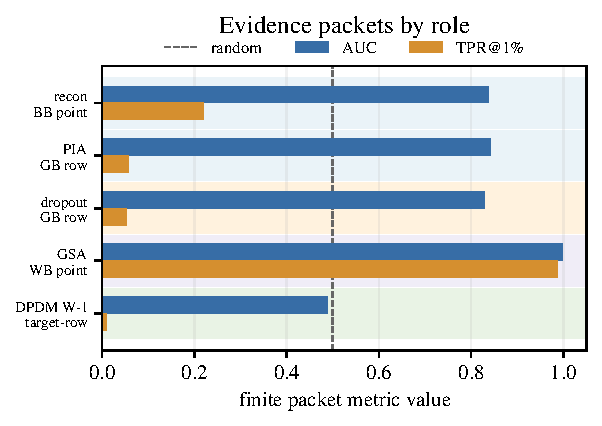
\includegraphics[width=\linewidth]{figures/admitted_rows_metrics.pdf}
\caption{AUC and TPR@1\%FPR for admitted rows. The figure compares evidence
under different access and defense contracts; it is not a single benchmark
leaderboard.}
\label{fig:admitted}
\end{figure}

\section{Output-Cloud Geometry Case Study}

The H2 response-strength cache contains repeated diffusion responses at
timesteps 40, 80, 120, and 160. Instead of comparing a query image directly to
outputs, the output-cloud scorer uses only geometry among outputs: within-step
repeat RMSE, cross-timestep centroid RMSE, and small response-cloud PCA/Gram
features. This design asks whether the response cloud itself carries
membership information.

On the existing 512/512 cache, output-cloud logistic scoring reaches AUC
0.9615, ASR 0.9004, TPR@1\%FPR 0.3340, and TPR@0.1\%FPR 0.1172. It improves on
raw H2 logistic by 0.0558 AUC and on lowpass H2 logistic by 0.0659 AUC. A label
shuffle returns random-level AUC 0.5076. Because the historical cache used
class-ordered seed offsets, DiffAudit released only a bounded shared-position
control: with identical per-position seed offsets for members and nonmembers,
the scorer still reaches AUC 0.9678 at seed 176 and 0.9562 at seed 177. A
fold-disjoint cross-cache transfer review gives AUC 0.9490 from seed 176 to
177 and AUC 0.9705 from seed 177 to 176.

\begin{figure*}[t]
\centering
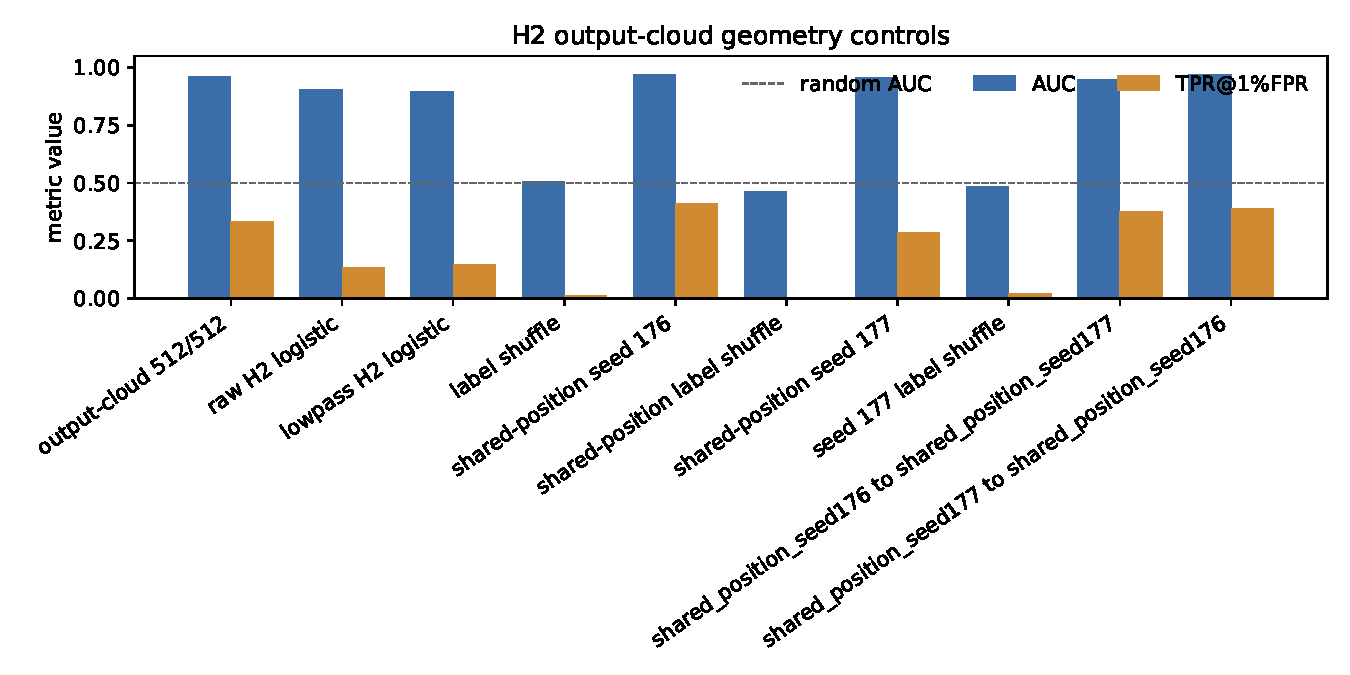
\includegraphics[width=\linewidth]{figures/h2_output_cloud_controls.pdf}
\caption{H2 output-cloud geometry controls. The signal beats raw/lowpass
baselines and survives label-shuffle, seed-offset control, seed stability, and
cross-cache transfer. It remains a research candidate because portability to
the SD/CelebA img2img contract is weak or not distinct from simple distance.}
\label{fig:h2}
\end{figure*}

The portability boundary is equally important. On the SD/CelebA img2img
admission cache, output-cloud geometry reaches only AUC 0.7888 with zero strict
tail recovery and underperforms the existing best simple-distance comparator by
0.088 AUC. A smaller stability cache is positive but still below simple
distance. Thus the paper reports output-cloud geometry as a controlled
mechanism candidate, not as an admitted black-box row.

\section{Negative and Support Evidence}

DiffAudit treats failed routes as measurement evidence when they answer a
specific decision question. ReDiffuse STL-10 provides exact public split
manifests and a locally scoreable bounded target, but fixed-timestep
denoising-loss is random-level (AUC 0.4996) and a SimA-style score-norm
observable remains weak (AUC 0.5053), even though ReDiffuse is a relevant
black-box diffusion MIA reference point~\cite{rediffuse2025}. CommonCanvas/CopyMark has a real 50/50
response contract, yet conditional denoising-loss reaches only AUC 0.5148.
Tracing the Roots feature tensors are positive (AUC 0.8158)~\cite{tracingroots2025}, but they are not
raw image-level evidence and lack target checkpoint/sample regeneration
artifacts for the current consumer boundary. The collaborator Stable Diffusion
ReDiffuse packet is replayable (AUC 0.7103), but source labels alone separate
members and nonmembers perfectly, so it is a cross-source stress test rather
than same-distribution membership evidence.

\begin{figure}[t]
\centering
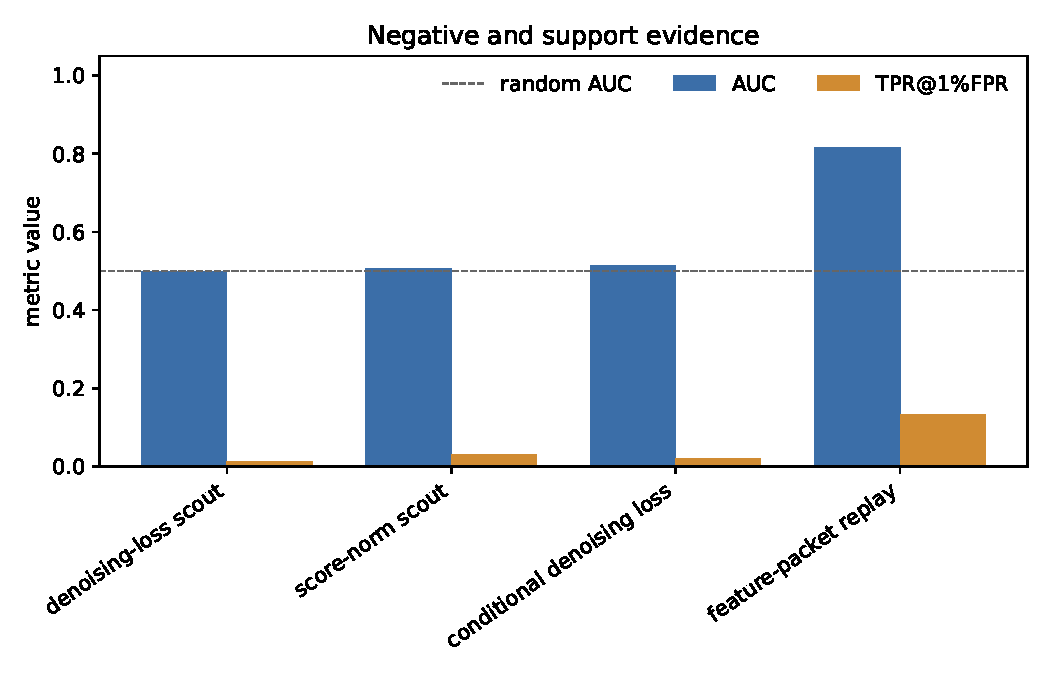
\includegraphics[width=\linewidth]{figures/negative_and_support_rows.pdf}
\caption{Negative and support evidence. These results are not failures of the
audit framework; they are examples of why scoreability, portability, and
consumer semantics must be separated.}
\label{fig:negative}
\end{figure}

\section{Discussion and Limitations}

The strongest criticism of DiffAudit is that evidence contracts may look like
engineering governance rather than research. We argue the opposite: in
diffusion membership inference, evidence contracts are part of the measurement
method. Without them, a high AUC can come from a source-label shortcut, a
prompt-conditioned auxiliary feature, a non-replayable score array, or a
finite-tail artifact. The H2 case study shows that DiffAudit can still discover
new technical signals; the contract simply controls how far those signals are
allowed to travel. This position is also consistent with broader caution that
membership inference alone should not be overstated as definitive proof of
training-data use~\cite{zhang2025cannotprove}.

This draft does not claim broad generalization across all diffusion models. It
does not claim that H2 output-cloud geometry is product-ready. It does not claim
that bounded weak scouts disprove the original methods they resemble. The next
scientific step for a full CCF-B+ submission is to add either a second
checkpoint-bound response asset for the output-cloud mechanism or a larger,
pre-registered public-artifact audit corpus for the evidence-contract
methodology.

\subsection{Threats to Validity}

\textbf{Internal validity.} Some results are produced by local replay scripts
and repository artifacts rather than by re-running complete upstream training
pipelines. DiffAudit mitigates this by recording row-level provenance and by
refusing to call bounded scouts full reproductions.

\textbf{External validity.} The admitted bundle is permission- and
asset-bound. It should not be read as evidence that every diffusion model leaks
at the same level, nor that one method dominates across modalities.

\textbf{Metric validity.} Low-FPR tails can be misleading on small packets. We
therefore report them as finite empirical readouts and keep packet size and
nonmember denominators attached to the claim.

\textbf{Publication bias.} Negative routes were selected because they affected
DiffAudit route decisions. A standalone reproducibility paper would need a
frozen corpus protocol before drawing broader conclusions about public artifact
availability.

\section{Conclusion}

DiffAudit turns diffusion membership inference from isolated score reporting
into evidence-contracted auditing. The current results show verified leakage
under admitted black-box, gray-box, and white-box contracts; reveal a promising
output-cloud response geometry signal; and document why many public artifacts
remain scientifically useful but non-admissible. This combination is the paper's
central point: publishable diffusion privacy evidence requires both strong
signals and strict claim boundaries.

\bibliographystyle{IEEEtran}
\bibliography{refs}

\end{document}
